\chapter{\IfLanguageName{dutch}{Stand van zaken}{State of the art}}%
\label{ch:stand-van-zaken}

% Tip: Begin elk hoofdstuk met een paragraaf inleiding die beschrijft hoe
% dit hoofdstuk past binnen het geheel van de bachelorproef. Geef in het
% bijzonder aan wat de link is met het vorige en volgende hoofdstuk.

% Pas na deze inleidende paragraaf komt de eerste sectiehoofding.

%Dit hoofdstuk bevat je literatuurstudie. De inhoud gaat verder op de inleiding, maar zal het onderwerp van de bachelorproef *diepgaand* uitspitten. De bedoeling is dat de lezer na lezing van dit hoofdstuk helemaal op de hoogte is van de huidige stand van zaken (state-of-the-art) in het onderzoeksdomein. Iemand die niet vertrouwd is met het onderwerp, weet nu voldoende om de rest van het verhaal te kunnen volgen, zonder dat die er nog andere informatie moet over opzoeken \autocite{Pollefliet2011}.

%Je verwijst bij elke bewering die je doet, vakterm die je introduceert, enz.\ naar je bronnen. In \LaTeX{} kan dat met het commando \texttt{$\backslash${textcite\{\}}} of \texttt{$\backslash${autocite\{\}}}. Als argument van het commando geef je de ``sleutel'' van een ``record'' in een bibliografische databank in het Bib\LaTeX{}-formaat (een tekstbestand). Als je expliciet naar de auteur verwijst in de zin (narratieve referentie), gebruik je \texttt{$\backslash${}textcite\{\}}. Soms is de auteursnaam niet expliciet een onderdeel van de zin, dan gebruik je \texttt{$\backslash${}autocite\{\}} (referentie tussen haakjes). Dit gebruik je bv.~bij een citaat, of om in het bijschrift van een overgenomen afbeelding, broncode, tabel, enz. te verwijzen naar de bron. In de volgende paragraaf een voorbeeld van elk.

%\textcite{Knuth1998} schreef een van de standaardwerken over sorteer- en zoekalgoritmen. Experten zijn het erover eens dat cloud computing een interessante opportuniteit vormen, zowel voor gebruikers als voor dienstverleners op vlak van informatietechnologie~\autocite{Creeger2009}.

%Let er ook op: het \texttt{cite}-commando voor de punt, dus binnen de zin. Je verwijst meteen naar een bron in de eerste zin die erop gebaseerd is, dus niet pas op het einde van een paragraaf.
\section{Machine Learning}

Machine Learning (ML) is een onderdeel van Artificial Intelligence (AI), een snel groeiend vakgebied op het raakvlak van data en statistiek dat feitgebaseerde beslissingen in verschillende sectoren aanstuurt \autocite{Jordan2015}. Door het toepassen van wiskundige principes kan Machine Learning verbanden leggen tussen gegevens om betrouwbare voorspellingen te genereren. Dit wordt mogelijk gemaakt door het gebruik van Machine Learning algoritmen, waarmee computers kunnen leren van data. Met iteratieve testen en validatie kunnen ze hun prestaties in de loop van de tijd verbeteren, waardoor ze nieuwe taken kunnen uitvoeren met nieuwe data \autocite{Shaveta2023}.\newline

\begin{figure}[h]
    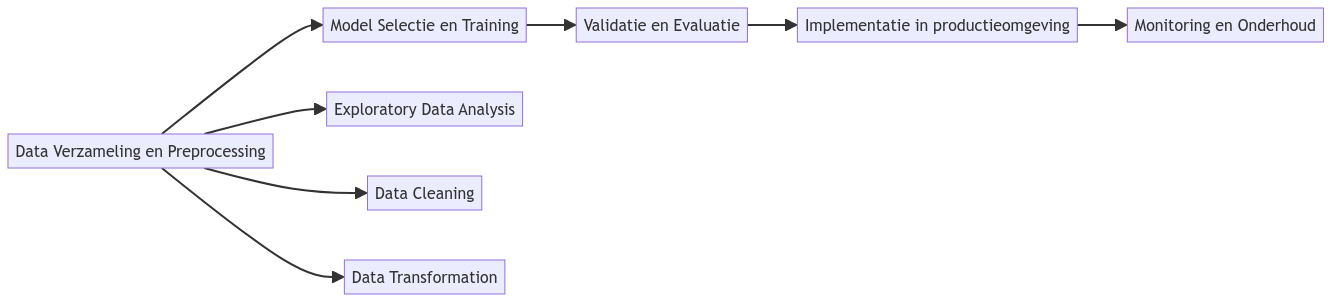
\includegraphics[width=\linewidth]{mlcycle.png}
    \caption{Machine Learning cycle}
    \label{fig:ML_cycle}
\end{figure}

Aldus \textcite{Schlegel2022} omvat de levenscyclus van een typisch Machine Learning-project verschillende fasen:

\begin{itemize}
    \item \textbf{Data Verzameling en Preprocessing:} relevante gegevens worden verzameld en voorbereid voor analyse, inclusief het reinigen van gegevens, het verwerken van ontbrekende waarden en het transformeren van gegevens naar een geschikt formaat voor Machine Learning-modellen.
    
    \item \textbf{Model Selectie en Training:} een geschikt Machine Learning-model wordt geselecteerd op basis van de aard van de gegevens en het projectdoel. Het model wordt getraind met behulp van verzamelde gegevens, waarbij parameters worden aangepast om een optimaal resultaat te bereiken.
    
    \item \textbf{Validatie en Evaluatie:} het getrainde model wordt gevalideerd met behulp van een aparte validatieset om de prestaties op nieuwe, niet eerder geziene data te beoordelen.
    
    \item \textbf{Implementatie in de Productieomgeving:} het model wordt geïmplementeerd om voorspellingen te genereren op nieuwe data, bijvoorbeeld door integratie in een bestaande softwareapplicatie of gegevensstroom.

    \item \textbf{Monitoring en Onderhoud:} het model wordt continu gemonitord om prestatieverlies of achteruitgang in nauwkeurigheid te detecteren. Indien nodig wordt het model opnieuw getraind met verse data om de prestaties te behouden of te verbeteren.
\end{itemize}

\subsection{Machine Learning Methoden}

Dit hoofdstuk richt zich op de verschillende methoden binnen het domein van Machine Learning (ML) die worden gebruikt om modellen te trainen en voorspellingen te genereren op basis van gegevens. Aan de hand van praktische voorbeelden en theoretische concepten worden de belangrijkste methoden binnen ML uitgelegd, waarbij de nadruk ligt op het begrijpen van hun toepassingen.

\begin{figure}[h]
    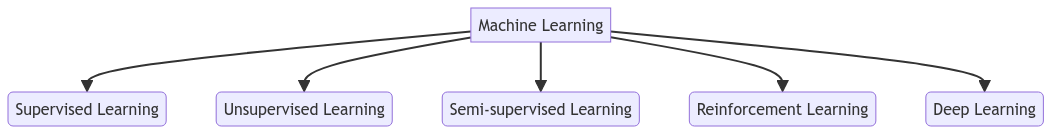
\includegraphics[width=\linewidth]{mm.png}
    \caption{Machine Learning en de subsets ervan}
    \label{fig:ML_subsets}
\end{figure}

Aldus \textcite{Mahesh2019} zijn verschillende soorten Machine Learning-methoden, waaronder:

\begin{itemize}
    \item Supervised Learning, waarbij het model wordt getraind op een dataset met gelabelde voorbeelden om een model te ontwikkelen voor nieuwe, niet eerder geziene data.

    \item Unsupervised Learning, waarbij het model wordt getraind op een dataset zonder gelabelde voorbeelden, om patronen en structuren in de data te ontdekken zonder voorafgaande kennis van de uitvoer.

    \item Semi-supervised Learning, die een combinatie van gelabelde en ongelabelde gegevens gebruikt voor training, om nauwkeuriger voorspellingen te maken.

    \item Reinforcement Learning, waarbij het model leert door interactie met een dynamische omgeving, om een optimale strategie te ontwikkelen om beloningen te maximaliseren.

    \item Deep Learning, een subset van Machine Learning die gebruikmaakt van kunstmatige neurale netwerken met meerdere lagen van verwerkingseenheden om complexe patronen in grote datasets te leren en te begrijpen.
\end{itemize}


Machine Learning speelt een cruciale rol in het genereren van inzichten uit gegevens en het maken van voorspellingen op basis van complexe patronen \autocite{Jordan2015}. Door de levenscyclus van Machine Learning-projecten te begrijpen en verschillende soorten Machine Learning-methoden te verkennen, kunnen onderzoekers en ontwikkelaars effectievere en nauwkeurigere modellen ontwikkelen om een breed scala aan problemen op te lossen.
%%%%%%%%%%%%%%%%%%%%%%%%%%%%%%%%%%%%%%%%%%%%%%%%%%%%%%%%%%%%%%%%%%%%%%%%%%%%%%%%%%%%%%%%%%%%%%%%%%%%%%%%%%%%%%%%%%
\section{CI/CD pipelines}

Een Continuous Integration/Continuous Deployment (CI/CD) pipeline is een cruciaal onderdeel van moderne softwareontwikkeling. Het versnelt en verbetert de betrouwbaarheid van de levering van webapplicaties. Een CI/CD pipeline bestaat uit een geordende reeks stappen die codewijzigingen automatisch integreren, testen en implementeren. Deze stappen omvatten Continuous Integration, Continuous Testing, Continuous Delivery en Continuous Deployment.

Dit is CI/CD pipelines uitgelegd zoals beschreven in \textcite{NaveenVemuri2024}:

Continuous Integration omvat het samenvoegen en testen van codewijzigingen van diverse ontwikkelaars om ervoor te zorgen dat de verschillende delen van de code goed samenwerken en geen conflicten veroorzaken.

Continuous Testing houdt in dat geautomatiseerde tests worden uitgevoerd om de functionaliteit en kwaliteit van de code te controleren. Dit zorgt ervoor dat eventuele fouten of bugs worden opgespoord voordat de code verder wordt verwerkt.

Vervolgens komt Continuous Delivery, waar de geteste code wordt voorbereid voor implementatie in de productieomgeving. Dit omvat vaak het compileren van de code en het gereedmaken van eventuele configuratiebestanden.

Tenslotte is er Continuous Deployment, waar de voorbereide code automatisch wordt gedeployed in de productieomgeving. Dit minimaliseert handmatige tussenkomst en verzekert een snelle en consistente implementatie van nieuwe code.\newline

\begin{figure}[h]
    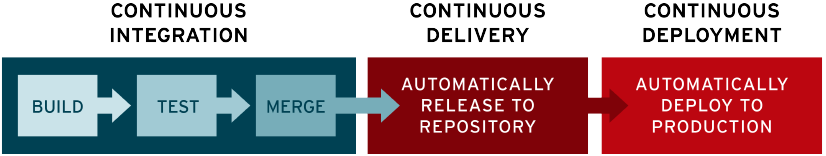
\includegraphics[width=\linewidth]{cdci.png}
    \caption{CI/CD Flow van \autocite{RedHat2023}}
    \label{fig:CICD_flow}
\end{figure}
  
%Figuur \ref{fig:CICD_flow} toont de flow van een CI/CD pipeline.

Binnen het domein van datamanagement benadrukken \textcite{Samad2018} en \textcite{Vadavalasa2020} de cruciale aspecten van het optimaliseren van beperkte datasets en de implementatie van Continuous Integration in de datapipeline. Ze tonen aan dat CI/CD pipelines een essentiële rol spelen bij het ontwikkelen van data-efficiënte ML-modellen en het waarborgen van de consistentie en betrouwbaarheid van datastromen.

CI/CD pipelines zijn een essentieel onderdeel van moderne softwareontwikkeling. Ze versnellen de levering van software, verhogen de kwaliteit en betrouwbaarheid, en bevorderen de samenwerking tussen teams. Datapipelines spelen een cruciale rol in ML door dataverwerking te automatiseren en de efficiëntie van modeltraining te verhogen.
%%%%%%%%%%%%%%%%%%%%%%%%%%%%%%%%%%%%%%%%%%%%%%%%%%%%%%%%%%%%%%%%%%%%%%%%%%%%%%%%%%%%%%%%%%%%%%%%%%%%%%%%%%%%%%%%%%
\section{Machine Learning Pipelines}

Het proces van het ontwikkelen van ML-modellen omvat een complexe reeks stappen, van het verzamelen en voorbereiden van data tot het trainen, evalueren en implementeren van modellen. Deze stappen zijn vaak repetitief en tijdrovend, wat de efficiëntie en schaalbaarheid van ML-projecten kan belemmeren.

Machine Learning pipelines zijn geautomatiseerde workflows die zijn ontworpen om deze stappen in de levenscyclus van een ML-project te stroomlijnen en te automatiseren. Ze bestaan uit een reeks geordende taken, zoals data-ingestion, data-preprocessing, feature engineering, modeltraining, modelbeoordeling en modelimplementatie. Deze pipelines zorgen voor consistente en gestructureerde uitvoering van deze taken, waardoor de ontwikkeling en implementatie van ML-modellen efficiënter worden.

De voordelen van Machine Learning pipelines zijn talrijk. Ten eerste verhogen ze de efficiëntie door repetitieve taken te automatiseren, waardoor de doorlooptijd van ML-projecten wordt verkort. Bovendien zorgen pipelines voor verbeterde reproduceerbaarheid, doordat ze garanderen dat experimenten op een consistente manier worden uitgevoerd, wat essentieel is voor wetenschappelijke validatie en het delen van resultaten. Verder bieden pipelines een betere schaalbaarheid door de implementatie van ML-modellen op grotere datasets en in productieomgevingen te vergemakkelijken. Ten slotte vergroten ze de transparantie van het ML-proces door de stappen in de workflow te documenteren en te volgen.

Pipelines kunnen worden geïmplementeerd met behulp van verschillende tools en frameworks, zoals Apache Airflow, Kubeflow, Kedro, MLflow, luigi en prefect. Deze technologieën bieden een gevarieerd scala aan mogelijkheden om de ontwikkeling en implementatie van pipelines te faciliteren en te optimaliseren, afhankelijk van de specifieke behoeften en vereisten van een project.

Al met al bieden Machine Learning pipelines een efficiënte en schaalbare manier om ML-modellen te ontwikkelen en te implementeren, waardoor de reproduceerbaarheid, transparantie en efficiëntie van ML-projecten worden bevorderd.

%%%%%%%%%%%%%%%%%%%%%%%%%%%%%%%%%%%%%%%%%%%%%%%%%%%%%%%%%%%%%%%%%%%%%%%%%%%%%%%%%%%%%%%%%%%%%%%%%%%%%%%%%%%%%%%%%%
\section{Frameworks}

Machine Learning pipelines zijn een cruciaal onderdeel van het Machine Learning proces \autocite{Jordan2015}. Ze automatiseren de stappen van dataverzameling en -voorbereiding tot modeltraining en -evaluatie, waardoor het efficiënter en reproduceerbaarder wordt.

Traditioneel worden Machine Learning pipelines uitgevoerd op cloudplatforms of op krachtige servers. Dit kan echter kostbaar zijn en vereist gespecialiseerde kennis. Lokale uitvoering van Machine Learning pipelines biedt een aantal voordelen:

\begin{itemize}
  \item Lagere kosten: Lokale uitvoering maakt gebruik van de eigen hardware van de gebruiker, wat de kosten van cloudresources kan besparen.
  \item Flexibiliteit: Gebruikers hebben meer flexibiliteit om te experimenteren met verschillende frameworks en configuraties.
\end{itemize}

Deze literatuurstudie onderzoekt de verschillende frameworks die beschikbaar zijn voor het lokaal uitvoeren van Machine Learning pipelines. We bespreken de voor- en nadelen van elk framework en geven richtlijnen voor het kiezen van het juiste framework voor deze onderzoeksvraag.
\subsection{Kedro}
\autocite{Kedro2024} is een open-source Python-bibliotheek die de ontwikkeling van betrouwbare, reproduceerbare en onderhoudbare Machine Learning-pipelines vereenvoudigt. Dit framework biedt een krachtige oplossing voor onderzoekers die lokaal uitgevoerde ML-pipelines willen opzetten en beheren.

Kedro bied verschillende pluspunten waaronder:
\begin{itemize}
    \item \textbf{Flexibiliteit en modulariteit:} Kedro maakt het mogelijk om ML-pipelines op een flexibele manier samen te stellen. Onderzoekers kunnen eenvoudig componenten toevoegen, verwijderen of aanpassen, waardoor ze zich kunnen aanpassen aan de veranderende behoeften van hun onderzoek.
    \item \textbf{Versiebeheer en reproduceerbaarheid:} Kedro integreert versiebeheer in ML-pipelines, waardoor experimenten reproduceerbaar worden en resultaten gevalideerd kunnen worden. Dit is cruciaal voor het bevorderen van transparantie en betrouwbaarheid in onderzoek.
    \item \textbf{Gegevenscatalogus:} Kedro biedt een geïntegreerde gegevenscatalogus waarmee onderzoekers datasets eenvoudig kunnen beheren, documenteren en traceren binnen de ML-pipeline. Dit vereenvoudigt het gegevensbeheer en bevordert de samenwerking tussen teamleden.
    \item \textbf{Lokale uitvoering:} Kedro ondersteunt lokale uitvoering van ML-pipelines, waardoor onderzoekers offline experimenten kunnen uitvoeren en ontwikkelen. Dit is met name gunstig voor onderzoek met gevoelige data of in situaties waar cloudresources niet beschikbaar zijn.
    \item \textbf{Integratie met populaire ML-frameworks:} Kedro integreert naadloos met populaire ML-frameworks zoals TensorFlow, PyTorch en scikit-learn. Hierdoor kunnen onderzoekers hun favoriete tools blijven gebruiken binnen de Kedro-pipeline.
    \item \textbf{Virtual environments:} Kedro ondersteunt het gebruik van virtual environments, waardoor onderzoekers afhankelijkheden kunnen isoleren en een gecontroleerde ontwikkelingsomgeving kunnen behouden.
    \item \textbf{Automatische documentatie:} Kedro kan automatisch gedetailleerde documentatie genereren voor ML-pipelines, inclusief informatie over datasets, parameters en dependencies.
    \item \textbf{Visualisatie:} Kedro biedt tools voor het visualiseren van ML-pipelines, waardoor onderzoekers een beter begrip krijgen van de gegevensstroom en de interacties tussen verschillende componenten.
\end{itemize}

Kedro heeft vele functionaliteiten maar er zijn enkele opmerkingen waarmee er rekening zou moeten gehouden worden:

\begin{itemize}
    \item \textbf{Leercurve:} Kedro heeft een zekere leercurve, hoewel de integratie met populaire ML-frameworks de overstap vereenvoudigt.
    \item \textbf{Opslagruimte:} Lokale uitvoering van ML-pipelines kan, afhankelijk van de datasetgrootte, veel opslagruimte vereisen.
    \item \textbf{Beperkte schaalbaarheid:} Kedro is primair gericht op lokale uitvoering en is mogelijk niet de beste keuze voor grootschalige ML-pipelines die op distributed computing-infrastructuur draaien.
\end{itemize}

De volgende code is een Machine Learning-pipelines in Kedro: 
    
Kedro is een krachtig framework voor onderzoekers die lokaal uitgevoerde ML-pipelines willen opzetten en beheren. De flexibiliteit, ondersteuning voor versiebeheer, geïntegreerde gegevenscatalogus en compatibiliteit met populaire ML-frameworks maken Kedro tot een waardevolle tool voor het lokaal uitvoeren van Machine Learning pipelines.

%%%%%%%%%%%%%%%%%%%%%%%%%%%%%%%%%%%%%%%%%%%%%%%%%%%%%%%%%%%%%%%%%%%%%%%%%%%%%%%%%%%%%%%%%%%%%%%%%%%%%%%%%%%%%%%%%%
\subsection{MLflow}
\autocite{MLflow2023} is een open-source Python-bibliotheek ontwikkeld door Databricks die een uitgebreide set functionaliteiten biedt voor het beheren van Machine Learning (ML)-projecten. De vier pijlers van MLflow zijn Tracking, Projects, Models en Registry.
\begin{itemize}
    \item \textbf{Tracking:} MLflow Tracking biedt een eenvoudige manier om experimenten te volgen en resultaten te vergelijken. Het registreert nauwkeurig relevante details gedurende de ML-levenscyclus, zoals code, parameters, metrieken en artefacten (modellen, datasets). Dit maakt het voor onderzoekers naadloos mogelijk om eerdere experimenten te reproduceren en verschillende configuraties te vergelijken.
    \item \textbf{Projects:} MLflow Projects zorgt voor een uniforme structuur voor ML-projecten en bevordert herbruikbaarheid. Onderzoekers kunnen gestandaardiseerde projectstructuren definiëren met MLflow Projects, waardoor consistente en reproduceerbare onderzoeksomgevingen worden gecreëerd.
    \item \textbf{Models:} MLflow Models biedt tools om modellen te verpakken en te implementeren in verschillende omgevingen. Het stroomlijnt de implementatie van ML-modellen in productieomgevingen door ze te verpakken in een gestandaardiseerd formaat, inclusief de modelcode, afhankelijkheden en configuratiedetails.
    \item \textbf{Registry:} MLflow Registry fungeert als een centrale hub voor het beheren van modelversies. Het stelt onderzoekers in staat om een gecentraliseerd repository in te stellen voor geregistreerde modellen, waardoor ze verschillende versies van modellen kunnen organiseren, volgen en openen.
\end{itemize}
MLflow biedt verschillende voordelen voor onderzoekers die zich bezighouden met ML-projecten:
\begin{itemize}
    \item \textbf{Verbeterde reproduceerbaarheid:} De zorgvuldige logging- en trackingmogelijkheden van MLflow garanderen dat experimenten gemakkelijk reproduceerbaar zijn, wat de geloofwaardigheid en betrouwbaarheid van onderzoek versterkt.
    \item \textbf{Gestroomlijnde samenwerking:} Gecentraliseerd model- en experimentbeheer bevordert naadloze samenwerking tussen onderzoekers, doordat ze elkaars werk eenvoudig kunnen delen en volgen.
    \item \textbf{Verbeterde efficiëntie:} MLflow automatiseert tijdrovende taken zoals experimenttracking en modelbeheer, waardoor onderzoekers waardevolle tijd kunnen vrijmaken voor kernonderzoeksactiviteiten.
    \item \textbf{Vereenvoudigde implementatie:} MLflow stroomlijnt het implementatieproces, waardoor onderzoekers hun modellen snel en efficiënt kunnen overbrengen van onderzoek naar productieomgevingen.
\end{itemize}
Er zijn enkele mogelijke nadelen verbonden aan het gebruik van MLflow voor het lokaal uitvoeren van Machine Learning pipelines:
\begin{itemize}
    \item \textbf{Complexiteit:} MLflow kan complex zijn om te installeren en te configureren, vooral voor onderzoekers die niet bekend zijn met Python of Databricks.
    \item \textbf{Vereist kennis:} MLflow vereist kennis van zowel Machine Learning als Python.
    \item \textbf{Beperkte integratie:} De integratie van MLflow met lokale tools en infrastructuur kan beperkt zijn.
    \item \textbf{Opslagruimte:} Het lokaal opslaan van alle experimentgegevens en artefacten kan veel opslagruimte vereisen.
\end{itemize}
De volgende code is een Machine Learning-pipelines in MLFlow: 

MLflow is een waardevolle tool voor onderzoekers die zich bezighouden met ML-projecten. Door reproduceerbaarheid te bevorderen, samenwerking te verbeteren en experimentatie, implementatie en beheer te stroomlijnen, stelt MLflow onderzoekers in staat om de kwaliteit en efficiëntie van hun onderzoeksinspanningen te verhogen.
%%%%%%%%%%%%%%%%%%%%%%%%%%%%%%%%%%%%%%%%%%%%%%%%%%%%%%%%%%%%%%%%%%%%%%%%%%%%%%%%%%%%%%%%%%%%%%%%%%%%%%%%%%%%%%%%%%
\subsection{Kubeflow}
\autocite{Kubeflow2021} is een open-source Machine Learning-toolkit die is ontworpen voor Kubernetes. Het biedt een krachtige infrastructuur voor onderzoekers om Machine Learning-pipelines op te zetten en te beheren in zowel lokale als cloudomgevingen.
Kubeflow biedt verschillende voordelen voor onderzoekers die zich bezighouden met het opzetten en beheren van Machine Learning-pipelines:
\begin{itemize}
    \item \textbf{Schaalbaarheid:} Door gebruik te maken van Kubernetes kan Kubeflow ML-workloads eenvoudig schalen, wat onderzoekers in staat stelt om snel te reageren op veranderende behoeften in hun onderzoek.
    \item \textbf{Geautomatiseerd beheer:} Kubeflow automatiseert de implementatie en het beheer van ML-pipelines, waardoor onderzoekers minder tijd hoeven te besteden aan handmatige configuratie en monitoring van infrastructuur, en zich meer kunnen richten op hun onderzoek.
    \item \textbf{Reproduceerbaarheid:} Met Kubeflow kunnen onderzoekers de omgeving vastleggen en de code versiebeheren, waardoor ze experimenten kunnen reproduceren en resultaten kunnen valideren, wat essentieel is voor de wetenschappelijke integriteit.
    \item \textbf{Flexibiliteit:} Kubeflow ondersteunt een breed scala aan ML-workloads, waardoor onderzoekers flexibel kunnen experimenteren met verschillende modellen en technieken binnen dezelfde infrastructuur, wat de innovatie stimuleert.
    \item \textbf{Integratie met Kubernetes:} Kubeflow is ontworpen om naadloos te integreren met Kubernetes, waardoor onderzoekers het gemakkelijk kunnen implementeren en beheren op lokale Kubernetes-clusters, wat de operationele efficiëntie verbetert.
    \item \textbf{Integratie met ML-frameworks:} Kubeflow biedt integratie met populaire ML-frameworks zoals TensorFlow, PyTorch en scikit-learn, waardoor onderzoekers hun favoriete tools kunnen blijven gebruiken binnen de Kubeflow-pipeline.
    \item \textbf{Monitoring:} Kubeflow biedt functionaliteiten voor het bijhouden en monitoren van ML-experimenten, waardoor onderzoekers inzicht krijgen in de prestaties van hun modellen en het gedrag van hun systemen kunnen volgen.
    \item \textbf{Model deployment:} Kubeflow ondersteunt model deployment en serving, waardoor onderzoekers hun modellen gemakkelijk kunnen delen en gebruiken in productieomgevingen.
\end{itemize}
Hoewel Kubeflow vele voordelen biedt, zijn er ook enkele potentiële nadelen waar onderzoekers rekening mee moeten houden:
\begin{itemize}
    \item \textbf{Complexiteit:} Kubeflow kan complex zijn om te installeren en te configureren, vooral voor onderzoekers die niet bekend zijn met Kubernetes, wat extra leer- en implementatietijd kan vereisen.
    \item \textbf{Vereist kennis:} Het effectief gebruik van Kubeflow vereist kennis van zowel Machine Learning als Kubernetes, wat een uitdaging kan zijn voor onderzoekers zonder ervaring in deze gebieden.
    \item \textbf{Beperkte ondersteuning:} De ondersteuning voor lokale uitvoering van Kubeflow is beperkter dan voor cloudomgevingen, wat mogelijk beperkingen kan opleggen aan onderzoekers die afhankelijk zijn van lokale resources.
\end{itemize}

Ondanks de mogelijke nadelen blijft Kubeflow een waardevol framework voor onderzoekers die schaalbare en flexibele ML-pipelines willen opzetten en beheren in lokale omgevingen. De voordelen zoals schaalbaarheid, geautomatiseerd beheer, ondersteuning voor reproduceerbare experimenten en integratie met populaire ML-frameworks maken Kubeflow tot een belangrijk instrument voor onderzoeksinspanningen.

%%%%%%%%%%%%%%%%%%%%%%%%%%%%%%%%%%%%%%%%%%%%%%%%%%%%%%%%%%%%%%%%%%%%%%%%%%%%%%%%%%%%%%%%%%%%%%%%%%%%%%%%%%%%%%%%%%
\subsection{ZenML}

\textcite{ZenML2024} is een open-source framework dat Python-gebaseerde Machine Learning (ML) pipelines definieert en beheert, met als doel een end-to-end oplossing te bieden voor het ontwikkelen, implementeren en beheren van dergelijke pipelines. Het framework biedt een geïntegreerde aanpak voor het opslaan van pipelines in een centrale repository, waardoor hergebruik en delen gemakkelijk worden gemaakt. Deze pipelines kunnen zowel lokaal als op afstand worden uitgevoerd, met ondersteuning voor verschillende platforms zoals Kubernetes en Docker.

Een kenmerk van ZenML is de uitgebreide monitoringfunctionaliteit die wordt geboden, waardoor onderzoekers en ontwikkelaars de voortgang en prestaties van hun pipelines nauwkeurig kunnen volgen. Bovendien maakt ZenML het mogelijk om pipelines efficiënt te herstarten vanaf een mislukte stap, waardoor de foutopsporingsprocedure wordt vereenvoudigd en versneld.

Een belangrijk aspect van ZenML is de integratie van MLOps-functionaliteit, inclusief artefactbeheer, versiebeheer en experimentenbeheer, waardoor het framework aantrekkelijk is voor teams die streven naar best practices op het gebied van Machine Learning operations.

In vergelijking met andere frameworks zoals Apache Airflow, Luigi en Kubeflow Pipelines, valt ZenML op vanwege zijn eenvoudige leercurve, flexibiliteit in configuratie en aanpassing, en zijn brede scala aan functionaliteiten. Bovendien onderscheidt ZenML zich door zijn expliciete focus op MLOps, waardoor het een waardevolle aanwinst is voor onderzoeksgemeenschappen en industriële toepassingen.

Als een robuust framework dat zich richt op gebruiksvriendelijkheid, schaalbaarheid en het implementeren van MLOps-best practices, is ZenML een geschikte keuze voor data scientists en Machine Learning engineers die streven naar een effectieve en efficiënte aanpak voor het beheren van ML pipelines.


%%%%%%%%%%%%%%%%%%%%%%%%%%%%%%%%%%%%%%%%%%%%%%%%%%%%%%%%%%%%%%%%%%%%%%%%%%%%%%%%%%%%%%%%%%%%%%%%%%%%%%%%%%%%%%%%%%
\subsection{Prefect}

\textcite{Prefect2024} is een open-source framework dat Python-gebaseerde ML pipelines definieert als gerichte acyclische grafieken (DAG's). Deze aanpak maakt het mogelijk om de stappen in de pipeline expliciet te definiëren en hun onderlinge afhankelijkheden te specificeren. Het framework biedt een breed scala aan functies voor het beheren en uitvoeren van pipelines, waaronder opslag, uitvoering, monitoring en het herstarten van pipelines vanaf een mislukte stap.

De voordelen van het gebruik van Prefect voor het lokaal uitvoeren van ML pipelines zijn aanzienlijk. Het framework biedt een intuïtieve interface die het gemakkelijk maakt om pipelines te definiëren en te beheren. Daarnaast is Prefect zeer schaalbaar en kan het pipelines uitvoeren op verschillende platforms, variërend van laptops tot clusters. Bovendien is Prefect flexibel configureerbaar om aan de specifieke behoeften van elk project te voldoen.

In vergelijking met andere frameworks voor het beheren van ML pipelines, zoals Apache Airflow, Luigi en Kubeflow Pipelines, onderscheidt Prefect zich door zijn gebruiksvriendelijkheid, flexibiliteit en uitgebreide functieset. Het heeft een eenvoudigere leercurve, is gemakkelijker aan te passen en biedt meer mogelijkheden dan zijn tegenhangers.

Ter afsluiting demonstreren we de praktische toepassing van Prefect met een proof of concept. We definiëren een eenvoudige ML pipeline die een iris-classificatiemodel traint en evalueert, en laten zien hoe deze lokaal kan worden uitgevoerd met Prefect. Deze PoC bevestigt dat Prefect inderdaad een eenvoudige en efficiënte manier biedt om ML pipelines lokaal uit te voeren.

In conclusie is Prefect een krachtig framework voor het beheren en uitvoeren van ML pipelines. Met zijn gebruiksvriendelijke, schaalbare en flexibele karakter is Prefect een uitstekende keuze voor data scientists en Machine Learning engineers die op zoek zijn naar een betrouwbare oplossing voor het beheren van hun ML workflows.
\subsection{Apache Airflow}

\textcite{ApacheAirflow2024}, een open-source platform ontworpen voor het orchestreren van workflows, richt zich voornamelijk op data pipelines en geniet een brede populariteit. Vooral binnen het domein van Machine Learning (ML) worden zijn voordelen duidelijk erkend. Deze omvatten flexibiliteit, schaalbaarheid, betrouwbaarheid en gebruiksgemak.

De flexibiliteit van Airflow komt voort uit zijn vermogen om pipelines te bouwen met diverse taken, zoals het laden van data, het uitvoeren van ML-modellen, en het opslaan van resultaten. Deze taakdiversiteit maakt het platform veelzijdig en aanpasbaar aan verschillende behoeften. Bovendien kan Airflow eenvoudig worden opgeschaald om pipelines te beheren met een groot aantal taken en datavolumes, waardoor het geschikt is voor grootschalige projecten. De betrouwbaarheid van Airflow is een cruciaal voordeel, aangezien het features biedt voor het omgaan met fouten en het herstarten van mislukte taken, waardoor pipelines robuuster en veerkrachtiger worden. Daarnaast biedt het platform een gebruiksvriendelijke interface voor het definiëren en beheren van pipelines, waardoor de complexiteit wordt verminderd en het gemakkelijker wordt om workflows te beheren.

Binnen het domein van Machine Learning kunnen Airflow-pipelines worden ingezet voor een reeks taken, waaronder data laden, data pre-processing, model training, model evaluatie, model deployment en model monitoring. Door gebruik te maken van Airflow voor ML pipelines, kunnen organisaties profiteren van verbeterde efficiëntie, verhoogde betrouwbaarheid, verbeterde schaalbaarheid en verbeterde reproduceerbaarheid. Het automatiseren van pipeline-uitvoering bespaart tijd en vermindert handmatige inspanningen, terwijl de betrouwbaarheid wordt verhoogd door de ingebouwde foutafhandelingsmechanismen van Airflow. Bovendien kan Airflow moeiteloos worden geschaald om te voldoen aan de eisen van groeiende datasets en complexere taken, terwijl het delen en coderen van pipelines de reproduceerbaarheid verbetert.

Niettemin brengt het gebruik van Airflow voor ML pipelines enkele nadelen met zich mee. Het platform heeft een steile leercurve en kan complex zijn om te configureren en te gebruiken. Daarnaast kan Airflow overhead toevoegen aan pipelines, wat de prestaties kan beïnvloeden. Daarom moet de beslissing om Airflow te gebruiken voor ML pipelines zorgvuldig worden afgewogen, rekening houdend met de specifieke behoeften en vereisten van het project \autocite{Harenslak2021}.

In conclusie, Apache Airflow vertegenwoordigt een krachtig platform voor het orchestreren van workflows, met een bijzondere focus op data pipelines. Zijn flexibiliteit, schaalbaarheid, betrouwbaarheid en gebruiksgemak maken het een aantrekkelijke keuze voor het lokaal uitvoeren van ML pipelines. Echter, potentiële gebruikers moeten zich bewust zijn van de leercurve en mogelijke overhead die gepaard kunnen gaan met het gebruik ervan, en deze afwegen tegen de voordelen die het biedt voor hun specifieke projectbehoeften.

\subsection{Luigi}

\textcite{Luigi2024}, een open-source Python-bibliotheek, biedt een krachtige oplossing voor het uitvoeren van complexe Machine Learning-pipelines op een schaalbare manier. Het kernconcept van Luigi draait om het definiëren van workflows als gerichte acyclische grafieken (DAG's), waarbij elke taak in de grafiek afhankelijk kan zijn van andere taken. Deze aanpak maakt het eenvoudig om pipelines te creëren die bestaan uit een groot aantal afzonderlijke stappen.

De voordelen van Luigi ten opzichte van andere frameworks voor het uitvoeren van Machine Learning-pipelines zijn duidelijk. Ten eerste is Luigi ontworpen met gebruiksgemak in gedachten, waardoor het eenvoudig is om pipelines te definiëren en te configureren. Het biedt handige functies die het beheren van pipelines vereenvoudigen. Daarnaast is Luigi schaalbaar en kan het draaien op clusters van machines, waardoor het automatisch taken parallel kan uitvoeren en workflows kan schalen naar grote datasets. Bovendien is het betrouwbaar, met functionaliteit die specifiek is ontworpen om robuust te zijn tegen fouten, waaronder het automatisch opnieuw uitvoeren van taken die mislukken en het herstellen van workflows van fouten.

Luigi is een veelgebruikte keuze voor het uitvoeren van Machine Learning-pipelines in verschillende omgevingen, zoals onderzoek en commerciële implementaties. Het wordt door onderzoekers gebruikt voor het uitvoeren van Machine Learning-experimenten en door bedrijven om pipelines in productie te nemen. Als open-source project heeft Luigi een actieve community van ontwikkelaars die bijdragen aan de verdere ontwikkeling en uitbreiding van de functionaliteit.

Hoewel Luigi Pipelines vaak wordt ingezet op clusters van machines, is het ook relevant voor het lokaal uitvoeren van ML pipelines. Dit kan voordelig zijn voor ontwikkeling en testen, vooral bij kleine datasets of wanneer gevoelige data betrokken is. Luigi vereenvoudigt het lokale uitvoeren van Machine Learning-pipelines door taken automatisch parallel uit te voeren op de lokale machine en workflows te herstellen van eventuele fouten.

Met een actieve ontwikkelingscommunity kunnen we verwachten dat Luigi Pipelines in de toekomst nog krachtiger en flexibeler zal worden. Dit maakt het een aantrekkelijke keuze voor zowel grootschalige implementaties als lokale uitvoeringen van Machine Learning-pipelines.
%%%% Apache Airflow: https://airflow.apache.org/
%%Luigi: https://luigi.readthedocs.io/en/stable/
%%%Kubeflow Pipelines: https://www.kubeflow.org/docs/pipelines/
%%% GITHUB PREFECT EN PREFECT DOCS BRON
\section{Risico Analyse}
Om te bepalen welk framework moet worden gebruikt, werd in samenwerking met de co-promotor een risicoanalyse opgesteld. Deze analyse omvat alle criteria die een framework moet hebben om te worden gebruikt in het opleidingsonderdeel ``Machine Learning Operations''.
De risicoanalyse bestaat uit twee delen: de ``must-haves'' en de ``should-haves''. De "must-haves" zijn criteria waaraan het framework absoluut moet voldoen. De ``should-haves'' omvatten de eigenschappen die wenselijk zijn voor een framework, maar niet essentieel zijn.
De must haves zijn:
\begin{itemize}
    \item De pipeline moet op eender welk besturingssysteem uitvoerbaar zijn (Windows, macOS en Linux)
    \item De omgeving waarin de pipeline uitgevoerd wordt is reproduceerbaar
    \item De pipeline moet uitvoerbaar zijn op een toestel dat voldoet aan de minimumvereisten van de opleiding
    \item De concepten van de pipeline kunnen vertaald worden naar een cloud omgeving (bv. Azure ML)
    \item De pipeline wordt beschreven in een leesbaar formaat (bv. YAML)
    \item De pipeline is in staat om lokaal uitgevoerd te worden, al dan niet met een minimalistisch model
\end{itemize}
De should haves zijn:
\begin{itemize}
    \item De pipeline kan in een container uitgevoerd worden
    \item De pipeline kan een rollback uitvoeren wanneer het model niet voldoet aan vooropgestelde criteria
\end{itemize}

Aan de hand van deze criteria zal besloten worden welke framework(s) gekozen zal worden om de Proof-of-Concept uit te werken.